\chapter{Game-Theoretic Evaluation Metrics}
\label{app:game-theory}

This appendix details the four game-theoretic metrics introduced in Section~\ref{subsec:game-theoretic} and summarized in Table~\ref{tab:metrics-summary}. All operate on the same pairwise win-rate matrix $W \in [0,1]^{n{\times}n}$, where $W_{ij}$ is the win rate of agent~$i$ against agent~$j$ and $n$ is the number of agents. Draws count as half a win for each side, and the diagonal is set to $0.5$ (no self-play). A four-agent worked example in Section~\ref{sec:illustrative-example} illustrates how the four metrics complement one another on the same matrix.

\section{Nash Averaging}
\label{app:nash-impl}

Nash averaging~\cite{balduzziReevaluatingEvaluation2018} answers the question: \hlc{gray!12}{``If an adversary could pick the worst-case opponent, which mix of agents minimizes the damage?''}

\medskip

Pairwise results are treated as a two-player zero-sum meta-game, where each ``player'' is not an agent but a \emph{selector} choosing which agent to deploy. The payoff matrix $A \in [-0.5,0.5]^{n{\times}n}$ centers the win-rate matrix around zero:
\begin{equation}
    A_{ij} = W_{ij} - 0.5
\end{equation}
so that $A_{ij} > 0$ means agent $i$ beats $j$ more than half the time.

The Nash equilibrium is the probability distribution $\mathbf{p}^* \in \Delta^{n-1}$\footnote{The probability simplex $\Delta^{n-1} = \{\mathbf{p} \in \mathbb{R}^n : p_i \geq 0, \sum_i p_i = 1\}$.} over the agent pool that guarantees the best possible payoff against the worst-case opponent choice. It is found by solving:
\begin{equation}
    \max_{v,\, \mathbf{p} \in \Delta^{n-1}} \; v
    \quad \text{s.t.} \quad
    \sum_{i} p_i \, A_{ij} \geq v \;\; \forall\, j
\end{equation}
Equivalently, $\mathbf{p}$ achieves expected payoff at least $v$ against every opponent $j$, with $v$ maximized.

The solution $\mathbf{p}^*$ gives the \emph{Nash weights}: agents with $p_i^* > 0$ form the \emph{equilibrium support}, while agents with $p_i^* = 0$ are redundant.

The \emph{Nash score} of each agent measures how well it performs against this optimal mix:
\begin{equation}
    s_i = \sum_{j} A_{ij} \, p_j^*
\end{equation}
An agent that only beats weak opponents (those with $p_j^* = 0$) scores low, while one that holds up against the strongest mix scores high. This makes Nash averaging robust to pool composition: adding clones or weak agents does not inflate scores.

\section{$\alpha$-Rank}
\label{app:alpharank-impl}

$\alpha$-Rank~\cite{omidshafieiARankMultiAgentEvaluation2019} answers the question: \hlc{gray!12}{``If agents competed in an evolutionary population, which strategies would survive and dominate over time?''}

\medskip

$\alpha$-Rank models a finite population of $m$ individuals where, at any moment, all play the same strategy (an agent from the pool). A random mutant appears playing a different strategy and either takes over the population or dies out. The ranking reflects which strategies are hardest to displace and most likely to invade others.

\paragraph*{Fitness.} Each individual's fitness is its average win rate against the rest of the population. When the population contains $k$ individuals playing strategy~$j$ and $(m - k)$ playing~$i$:
\begin{equation}
    f_j(k) = \frac{(k-1)\,W_{jj} + (m-k)\,W_{ji}}{m-1},
    \qquad
    f_i(k) = \frac{k\,W_{ij} + (m-k-1)\,W_{ii}}{m-1}
\end{equation}

\paragraph*{Fixation probability.} Under Fermi selection dynamics, the probability that a single $j$-mutant takes over a population of $i$-players is:
\begin{equation}
    \rho_{i \to j} = \left( 1 + \sum_{k=1}^{m-1} \exp\!\left( \sum_{\ell=1}^{k} -\alpha \bigl( f_j(\ell) - f_i(\ell) \bigr) \right) \right)^{-1}
\end{equation}
where $\alpha$ controls selection pressure. When $\alpha \to 0$, mutations reach fixation at random ($\rho_{i \to j} = 1/m$); when $\alpha \to \infty$, only strictly superior strategies invade.

\paragraph*{Markov chain.} With uniformly random mutants, the transition matrix between strategies is:
\begin{equation}
    T_{ij} =
    \begin{cases}
        \dfrac{\rho_{i \to j}}{n - 1} & \text{if } i \neq j \\[6pt]
        1 - \displaystyle\sum_{k \neq i} T_{ik} & \text{if } i = j
    \end{cases}
\end{equation}
Each off-diagonal entry $T_{ij}$ is the probability that strategy $j$ invades and replaces $i$. The diagonal $T_{ii}$ is the probability that no mutation succeeds and strategy $i$ persists.

\paragraph*{Ranking.} The $\alpha$-Rank score of each agent is its entry $\pi_i$ in the stationary distribution $\boldsymbol{\pi}$ satisfying $\boldsymbol{\pi}^\top T = \boldsymbol{\pi}^\top$: the long-run fraction of time the population spends playing strategy $i$. The agent with the largest $\pi_i$ is ranked first and dominates the evolutionary dynamics. Unlike Nash averaging, $\alpha$-Rank always produces a unique ranking, even when multiple equilibria exist.

\section{Copeland Score}
\label{app:copeland-impl}

The Copeland score~\cite{saariCopelandMethodRelationships1996} answers the question: \hlc{gray!12}{``How many opponents does the agent beat head-to-head, regardless of margin?''}

\medskip

Each pairwise matchup is reduced to a sign:
\begin{equation}
    c_{ij} =
    \begin{cases}
        +1 & \text{if } W_{ij} > 0.5 \quad \text{(win)} \\
        \phantom{+}0 & \text{if } W_{ij} = 0.5 \quad \text{(draw)} \\
        -1 & \text{if } W_{ij} < 0.5 \quad \text{(loss)}
    \end{cases}
\end{equation}

The Copeland score of agent~$i$ is then:
\begin{equation}
    C_i = \sum_{j \neq i} c_{ij}
\end{equation}

Scores range from $-(n-1)$ to $+(n-1)$. An agent achieving $C_i = +(n-1)$ beats every opponent and is a \emph{Condorcet winner}. Since margin is discarded (both 51\% and 99\% wins yield $c_{ij} = +1$), the Copeland score measures dominance breadth.

\section{Regret}
\label{app:regret-impl}

Regret~\cite{savageTheoryStatisticalDecision1951} answers the question: \hlc{gray!12}{``For each opponent, how much worse is this agent compared to the best agent in the pool?''}

\medskip

Adapted from the minimax regret criterion, the regret of agent~$i$ against opponent~$j$ is the gap between $i$'s win rate and the pool's best win rate against $j$:
\begin{equation}
    r_{ij} = \max_{k} W_{kj} - W_{ij}
\end{equation}

Two summaries are reported:
\begin{align}
    \text{Average regret}(i)    &= \frac{1}{n-1} \sum_{j \neq i} r_{ij} \\
    \text{Worst-case regret}(i) &= \max_{j \neq i} \; r_{ij}
\end{align}

Lower values are better in both cases. An agent with zero average regret is the best choice against every opponent. An agent with high worst-case regret has a single matchup where it performs much worse than the best available alternative, a weakness an adversary could exploit.

\section{An Illustrative Example}
\label{sec:illustrative-example}

Figure~\ref{fig:metrics-comparison} illustrates this complementarity on a four-agent example whose matrix $W$ contains a non-transitive cycle ($A$ beats $B$, $B$ beats $C$, $C$ beats $A$) together with a fourth agent $D$ whose only victory is over $C$. The four metrics yield four complementary perspectives on the same matrix.\emph{(i)}~\textbf{Copeland} ties $A$ and $B$ at the top ($+1$) and $C$ and $D$ at the bottom ($-1$), too coarse to separate within either tier despite $A$ beating $B$ and $D$ beating $C$ head-to-head. \emph{(ii)}~\textbf{Nash} scores each agent by its expected payoff against the equilibrium mixture: $A$, $B$, and $C$ tie at exactly $0$, the value of the game, forming the non-exploitable frontier, while $D$ falls to $-0.08$ as a dominated strategy never played at equilibrium. Nash thus separates $C$ from $D$ where Copeland lumps them together, but leaves the frontier itself unranked. \emph{(iii)}~\textbf{$\alpha$-Rank} resolves that frontier through simulated evolutionary invasion, ranking $A > B > C$ ($\pi = 0.41,\,0.32,\,0.21$ for $A,B,C$; $\alpha = 1$, $m = 50$), as a population of $A$ resists invading mutants more reliably than one of $B$ or $C$. \emph{(iv)}~\textbf{Average regret}, the gap to the best response against each opponent, leaves $A$ and $B$ nearly identical ($0.12$ vs $0.13$): $B$'s two suboptimal matchups have small gaps ($0.30$ and $0.10$), whereas $A$'s single one against $C$ is larger ($0.35$). Each panel thus exposes something the others miss, only $\alpha$-Rank resolving $A$'s dominance and only Nash distinguishing the non-exploitable $C$ from the dominated $D$, which motivates reporting the four jointly.

\begin{figure}[!ht]
    \centering
    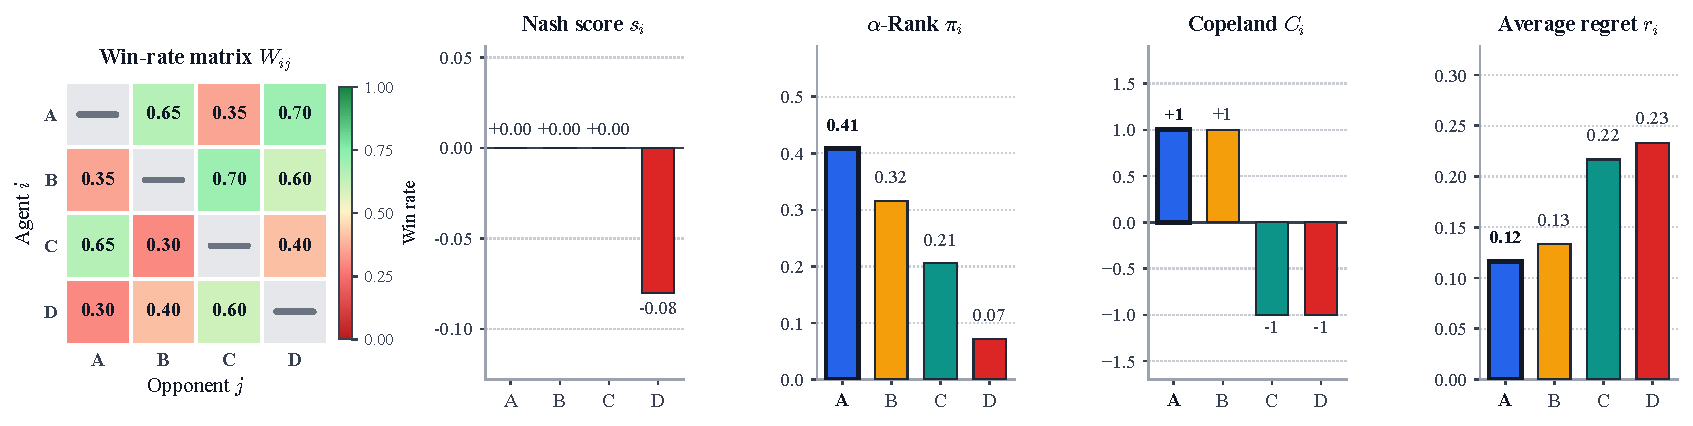
\includegraphics[width=\linewidth]{chapters/appendix/figures/metrics_comparison.pdf}
    \caption[Four tournament metrics on a $4$-agent example]{Complementarity of the four tournament metrics on a small $4$-agent example. The pairwise win-rate matrix $W$ (left) is the input to all four metrics (right): Nash score $s_i$, $\alpha$-Rank $\pi_i$, Copeland score $C_i$, and average regret $r_i$.}
    \label{fig:metrics-comparison}
\end{figure}